\section{Technical Difficulties}
\label{sec:tech-diff}

\subsection{Image Rotation}
\label{ssec:trans}

One issue which was faced when creating the large .pgm file containing all the input images, was that they were rotated 90\degree to the right, as demonstrated in Figure \ref{fig:rotated-input}.

\begin{figure}[H]
  \centering
  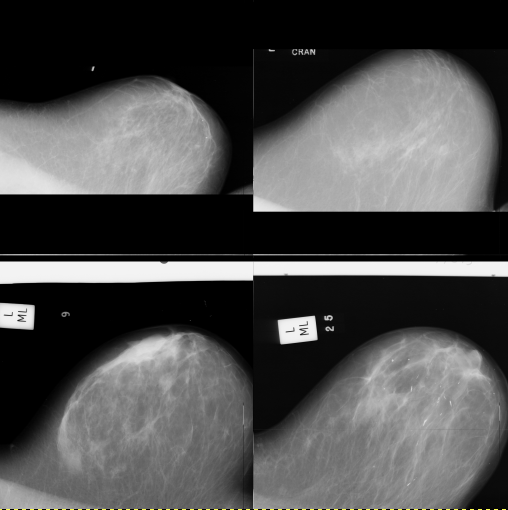
\includegraphics[width=0.4\textwidth]{Chapter2/technical-img/rotation.png}
  \caption{4 rotated input images concatenated into one larger image.}
  \label{fig:rotated-input}
\end{figure}

It quickly became apparent that the order in which the image array was being written to file to create this larger pgm file was incorrect, however due to MATLAB's clever use of vectorisation, it was difficult to diagnose where the issue lay. After some investigation, it was revealed that the function \texttt{fwrite} by MATLAB \cite{fwrite}, used for writing binary data to file, wrote each line out column-by-column, rather than the customary row-by-row approach.

To mitigate this issue, the array passed into fwrite would have to be transposed prior or during being passed into the function. There are two ways in which MATLAB permits the \gls{transposition} of arrays:

\subsubsection{Simple 2D array transposition}

MATLAB has a \say{Transpose} function which simply flips two elements in a 2D array as utilised in:

\begin{lstlisting}[style=Matlab-editor,frame=single]
    fwrite(output,handles.finalImg.','uchar');
\end{lstlisting}

Where handles.finalImg is a GUI holder for a 2D array of pixel values. This example was taken from the \texttt{removeMarker.m}  function - where the user can remove Medical Markers and save the output back to the original file.

\subsubsection{3D+ array transposition}

For arrays with more than 2 dimensions, simply swapping the values around will not work, so the MATLAB function \texttt{permute} \cite{permute} must be used.

\begin{lstlisting}[style=Matlab-editor,frame=single]

  sers=zeros(squareImageSize(1),squareImageSize(2),noOfScans); %set size of array

  for i = 1:noOfScans

    scan = fopen(strcat(pathname,'/',scanDirectory(i).name)); %open each input image individually
    im=(fread(scan,[squareImageSize(1),squareImageSize(2)],'uchar'));
    sers(:,:,i) = im; %add each input image to a 3D array which compiles all the input images into one

  end

outfname=sprintf('%s/big_scan.pgm', pathname);
s=sers(:,:,:);
saveSeries(outfname,permute(s,[2,1,3])); %use the saveSeries demo function to write the final image arrays out to a file

\end{lstlisting}

This example was taken from the \texttt{pgm2bigPgm.m} function - where a set of input images are passed in, and a large pgm image containing all the input images is outputted (as in Figure \ref{fig:final-output-4}). This image is then passed into the \Gls{Congealing} algorithm for alignment.

\subsubsection{Final Outcome}

After transposing all arrays which are to be saved out to file, whether directly through \texttt{fwrite} or \texttt{saveSeries}, all images are saved in the correct orientation.

\begin{figure}[H]
  \centering
  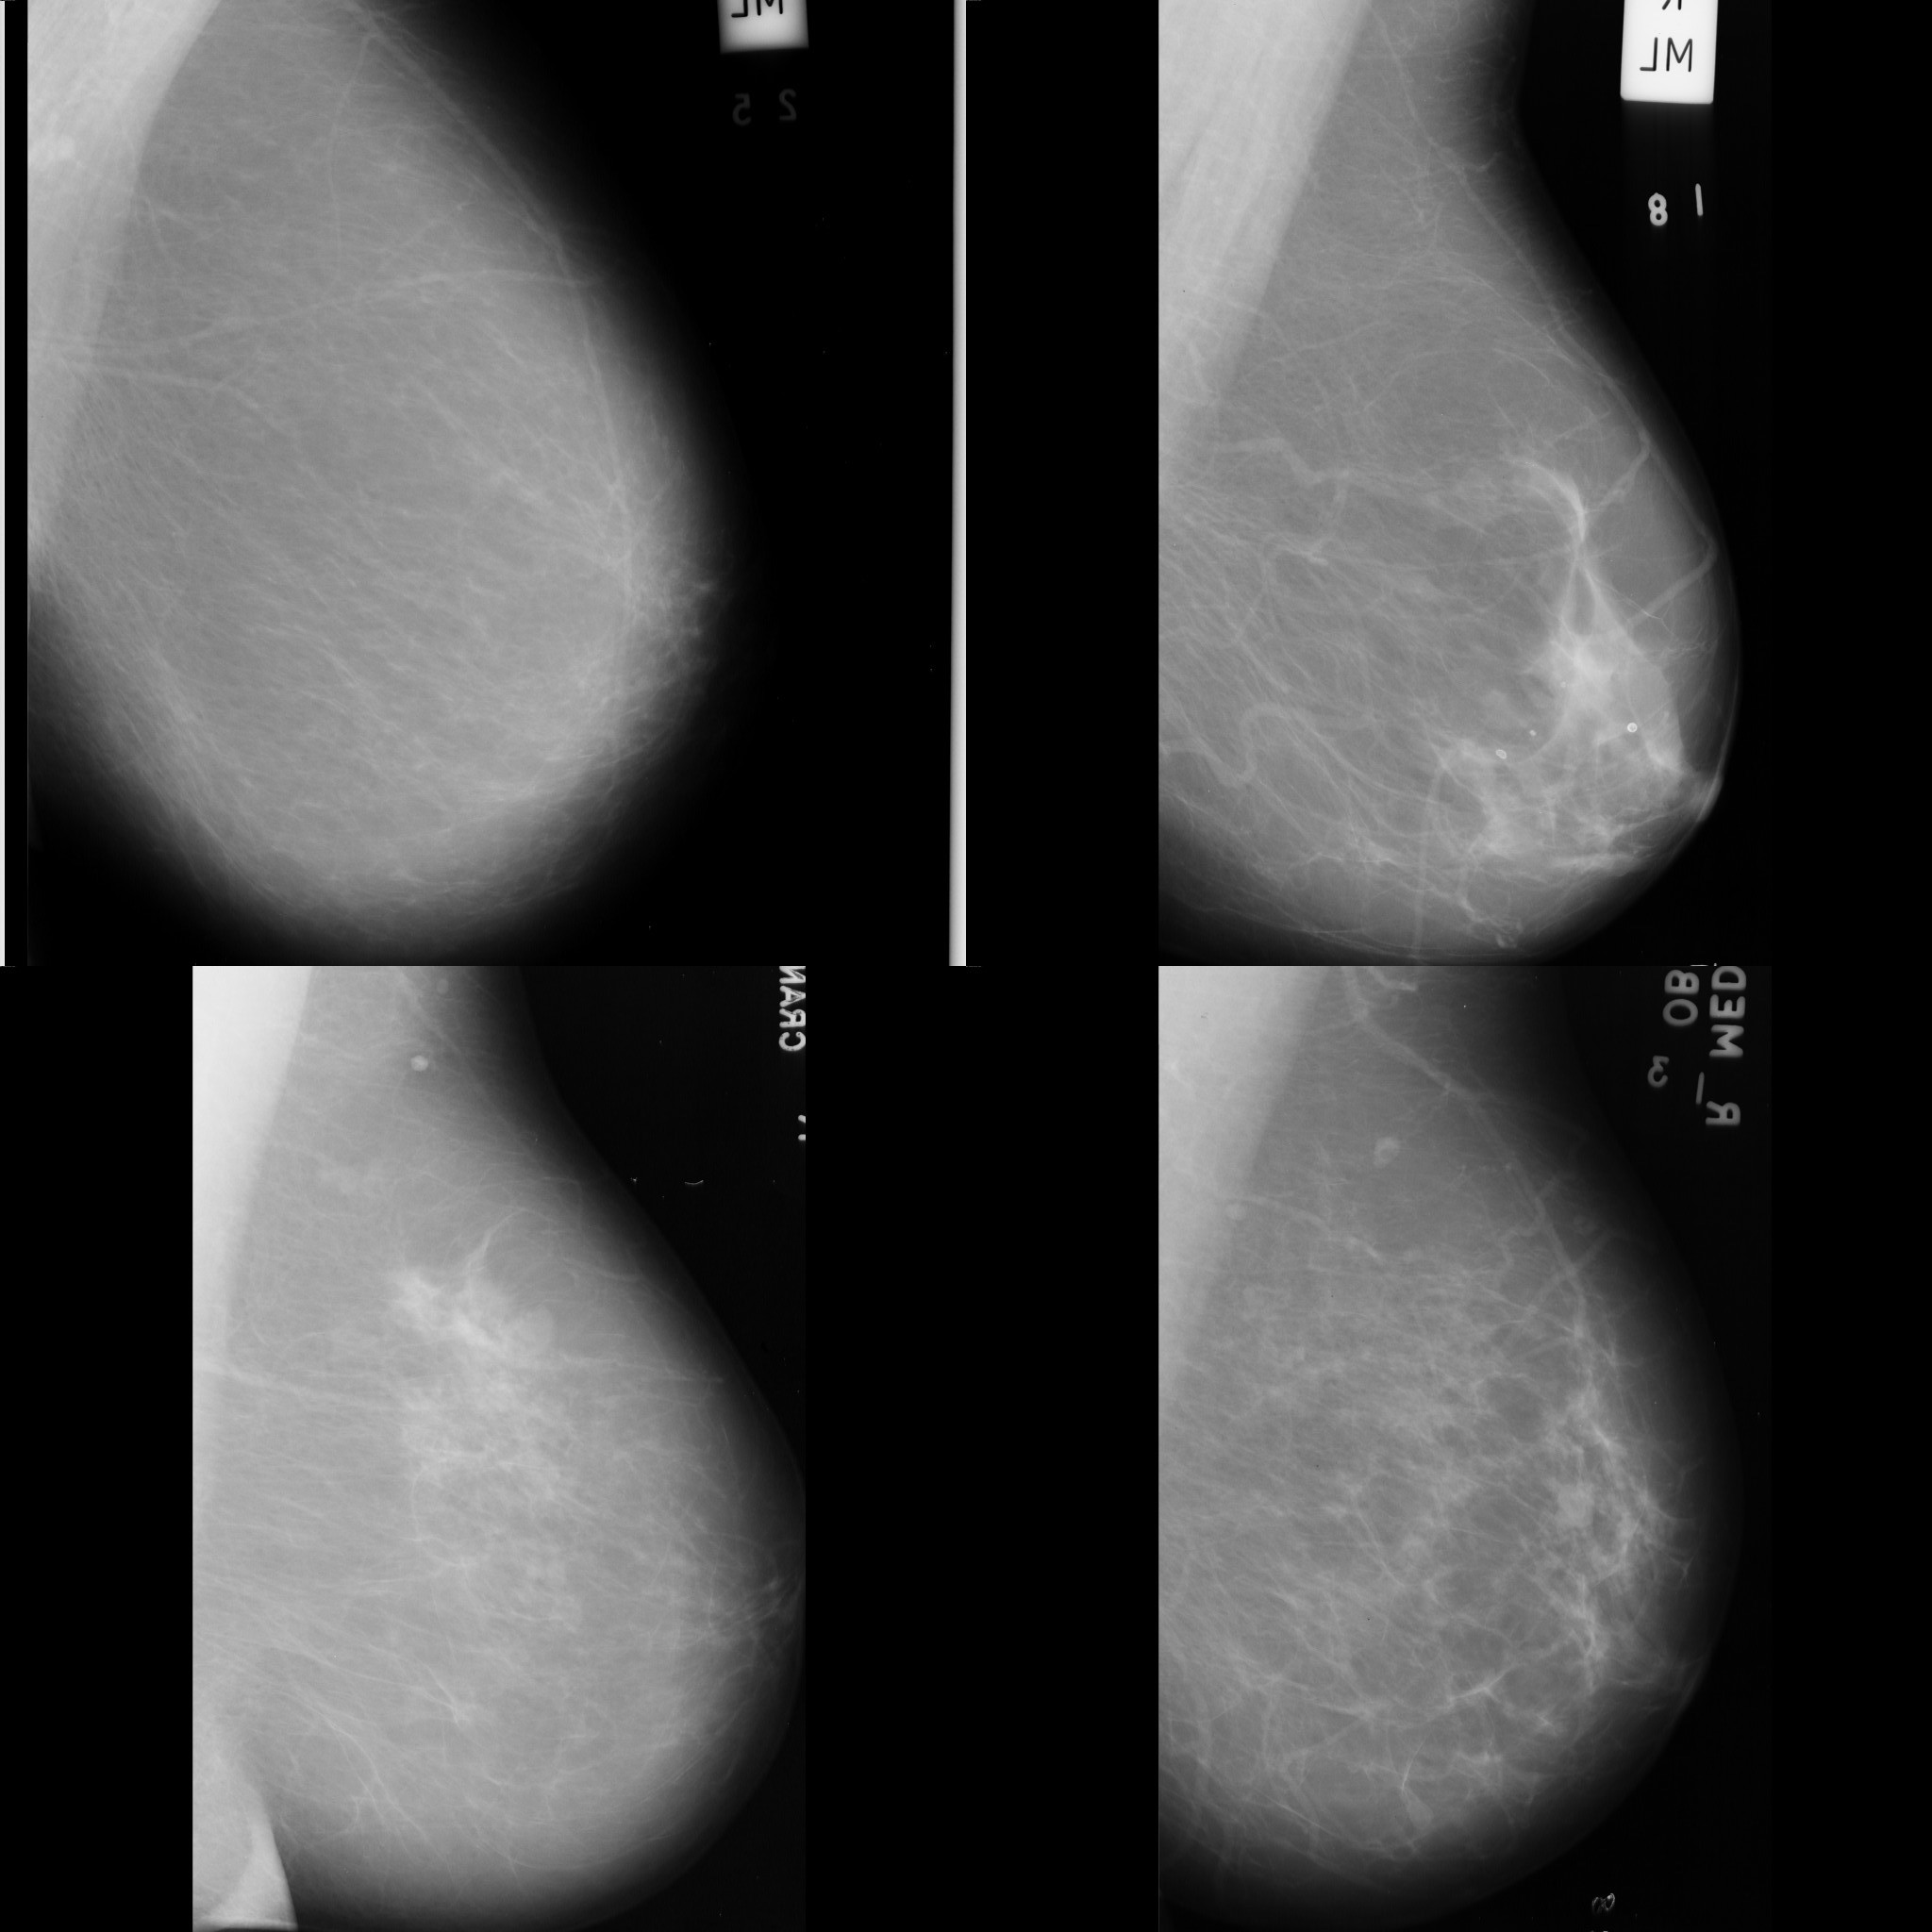
\includegraphics[width=0.4\textwidth]{Chapter2/technical-img/big_scan.jpg}
  \caption{Final output image.}
  \label{fig:final-output-4}
\end{figure}

\subsection{Medical Marker Removal}

This subsection has been formalised from a blog post written on 28th March 2016 \cite{Collins_2016}.

As the images are aligned using a comparison of the pixel-value, the Medical Markers included on mammograms cause an issue. This is because if more than one scan contains these white patches (left by the metal clip during scanning), then they will try and align with each other during the \Gls{Congealing} process.

\begin{figure}[H]
  \centering
  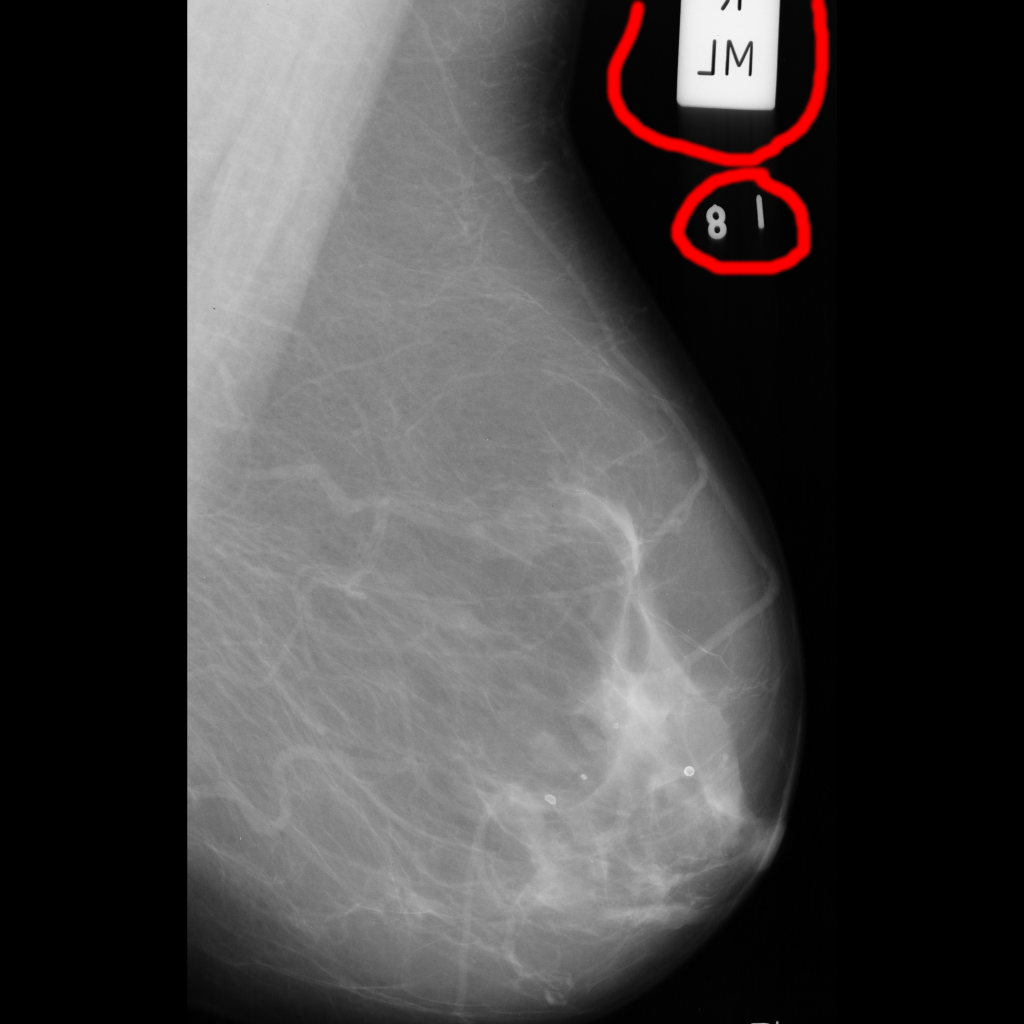
\includegraphics[width=0.4\textwidth]{Chapter2/technical-img/mdb196.png}
  \caption{Image containing Medical Markers}
  \label{fig:med-markers}
\end{figure}

Two options were available for the avoidance of Medical Markers:
\begin{itemize}
  \item Ask the User not to use scans containing Medical Markers
  \begin{itemize}
    \item This is extremely restrictive
    \item This could massively reduce their number of usable scans
  \end{itemize}
  \item Find a computer vision and/or image processing technique to remove these clips
  \begin{itemize}
    \item Preferably automatically
    \item Manually removing would work for small input data sets
  \end{itemize}
\end{itemize}

\subsubsection{Discarded ideas}

\begin{figure}[H]
    \centering
    \begin{subfigure}[t]{0.3\textwidth}
        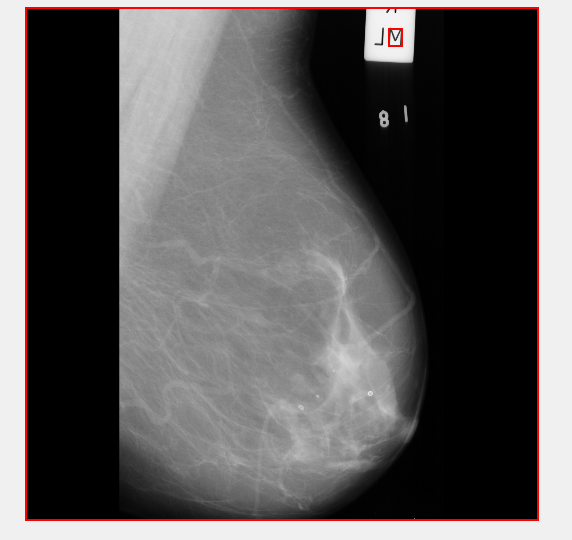
\includegraphics[width=\textwidth]{Chapter2/technical-img/morph.png}
        \caption{Squares detected in a mammogram using morphological operations.}
        \label{fig:morph}
    \end{subfigure} \hfill
    ~ %add desired spacing between images, e. g. ~, \quad, \qquad, \hfill etc.
      %(or a blank line to force the subfigure onto a new line)
    \begin{subfigure}[t]{0.3\textwidth}
        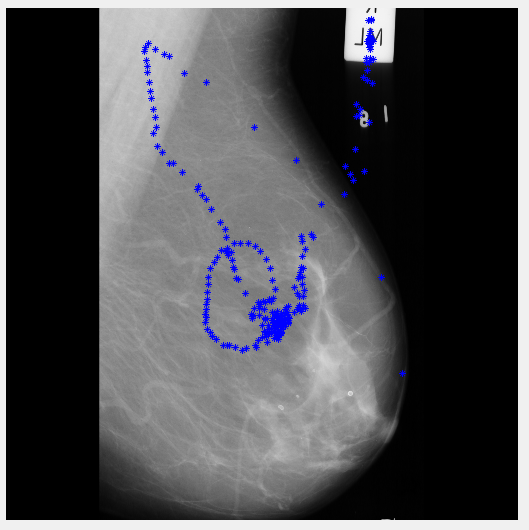
\includegraphics[width=\textwidth]{Chapter2/technical-img/regionprops.png}
        \caption{Regionprops detecting areas and superimposing the area information on a mammogram.}
        \label{fig:regionprops}
    \end{subfigure} \hfill
    \begin{subfigure}[t]{0.3\textwidth}
      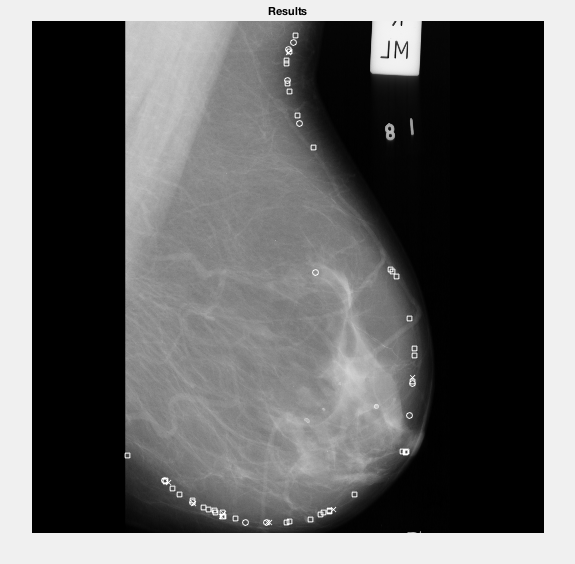
\includegraphics[width=\textwidth]{Chapter2/technical-img/shape_recog.png}
      \caption{Shape recognition picking out the rough boundary of breast tissue.}
      \label{fig:shape-recog}
    \end{subfigure}
    ~ %add desired spacing between images, e. g. ~, \quad, \qquad, \hfill etc.
    %(or a blank line to force the subfigure onto a new line)

    \begin{subfigure}[t]{0.3\textwidth}
      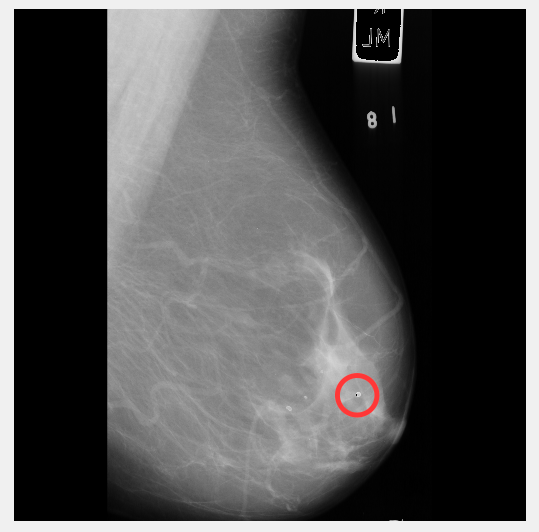
\includegraphics[width=\textwidth]{Chapter2/technical-img/remove-white-220.png}
      \caption{Removing areas of grey-level value above 220.}
      \label{fig:remove-white}
    \end{subfigure} \hfill
    \begin{subfigure}[t]{0.3\textwidth}
      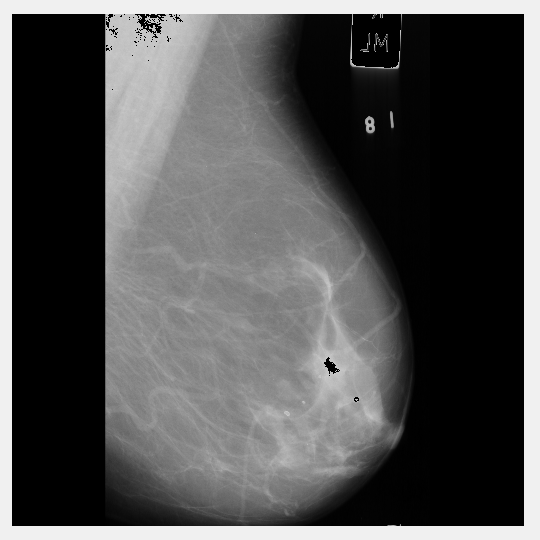
\includegraphics[width=\textwidth]{Chapter2/technical-img/remove-white.png}
      \caption{Lower grey-level removal threshold to 200.}
      \label{fig:remove-white-200}
    \end{subfigure} \hfill
    \begin{subfigure}[t]{0.3\textwidth}
      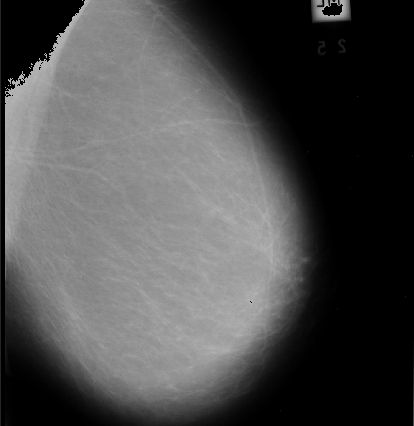
\includegraphics[width=\textwidth]{Chapter2/technical-img/other-scan.png}
      \caption{Applying removal over 220-value to another scan.}
      \label{fig:remove-other-scan}
    \end{subfigure}
    \caption{Output of discarded methods of marker removal}
    \label{fig:marker-removal-discards}
\end{figure}

\textbf{Morphological operation - remove squares from image}

Utilising a morphological operation, such as the one demonstrated by Chandra Kurniawan in the thread \cite{detect_square}. However, as can be seen in Figure \ref{fig:morph}, not only is the Marker itself not perfectly square, but because the image is square, it detects that instead. So removal would be made more difficult by the fact you would have to specify a maximum size square to remove, that smaller than the image size.

This idea was discarded due to the marker unlikely to ever be perfectly square in the scan.

\textbf{MATLAB function regionprops}

Another candidate function for removing Medical Markers was the MATLAB function \texttt{regionprops} \cite{regionprops}. The idea behind using this function would be to measure the area of the squares in the image, so then they could be removed. However, the output, as seen in Figure \ref{fig:regionprops}, was not something desired, and without spending an inordinate amount of time tweaking the function, it is not useful to the detection of the markers.

\textbf{Shape recognition demo}

On the Mathworks File Exchange site, a community run to help MATLAB users, there was a demo created by Ahmed Samieh to aid in the recognition of certain shapes \cite{shape_recognition}. It classifies the shape by properties such as roundness, ratios of dimensions and centroids.

Modifying this demo slightly to make it compatible with the grey-scale mammograms, the output is somewhat promising, as seen in Figure \ref{fig:shape-recog}.

However, due to the slightly inaccurate identification of the tissue boundary, this is likely to remove data which is useful to the \Gls{Congealing} algorithm. Unless this can become a near perfect outline around the breast tissue, it is unlikely to be useful for selecting and focusing in the object of interest.

\textbf{Removing white objects over a specified grey-level value}

Back on the Mathworks forum, there is a thread about removing white glare from a jewellery photo \cite{remove_white}. This was adapted to detect the medical marker by specifying to find and remove patches over 220 grey-level value. As seen in Figure \ref{fig:remove-white}, most of the marker has been removed, however it also removes a small bit of breast tissue.

To see if the entire marker could be removed, if you lower the grey-level threshold for removal to anything over 200 value, then the output is as in Figure \ref{fig:remove-white-200}. Unfortunately it does not remove the entire marker, and some of the vital breast tissue is lost.

Further to that, by running the white removal at grey-level value at 220 (the suitable choice for my first test scan) on another test scan and absolutely nothing is removed. Lower the threshold to begin removing white areas (down to grey-level value of 180) the results are less desirable, as demonstrated in Figure \ref{fig:remove-other-scan}.

\subsubsection{Chosen method}

Another demo on the MATLAB forum outlined a way in which a user can draw an area to remove, then a mask can be applied over the top to hide any problem areas (such as the Medical Markers) \cite{binary_mask}.

After reading through the demo given as an answer by \say{Image Analyst} on the forum, I rewrote the function in order to fit the removal criteria. The User can utilise the MATLAB function \texttt{imfreehand} \cite{imfreehand} to draw over the input image in order to indicate the area to be removed. This area is then filled in with the darkest grey-level value found in the drawn area (typically 0 for black, however may differ between scans).

\begin{figure}[H]
  \centering
  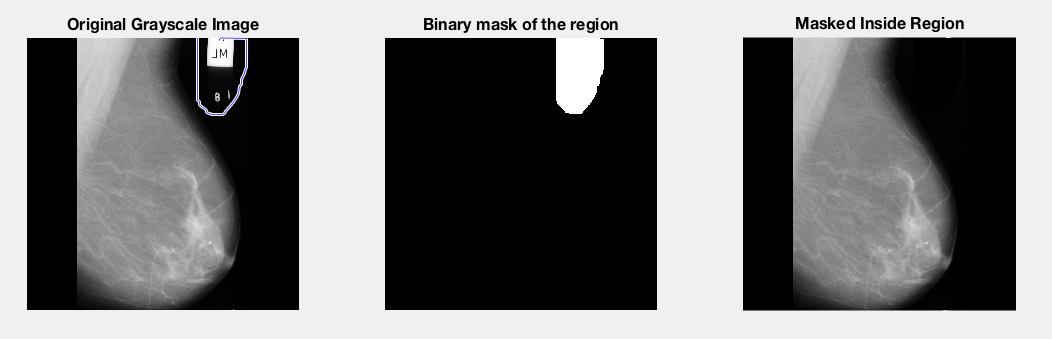
\includegraphics[scale=0.4]{Chapter2/technical-img/draw-to-remove.png}
  \caption{Image depicting the steps taken to remove Medical Markers from a scan.}
  \label{fig:remove-marker}
\end{figure}

As shown in Figure \ref{fig:remove-marker} this has been shown to be extremely successful and therefore was utilised in the project.

\subsection{.pgm file header}

As this project was building upon the work done by Learned-Miller \cite{joint-alignment}, it was useful to utilise the load function that was already in place. However, the nature in which the image files were loaded into the system caused some unexpected hurdles.

In order to understand how the demo data was uploaded, and therefore implement a function to compile a large set of mammogram scans in the correct format, research was carried out into the nature of \acrshort{pgm} files, and the function which comments play in the headers.

\subsubsection{PGM file format}

\acrfull{pgm} file format is part of a package called Netpbm, which contains 220 separate programs for dealing with files such as \acrshort{pgm}, pbm and pnm. As the name suggests, it is a lightweight-greyscale image format, which is simple for use in programs, making it ideal for this project.

The structure of \acrshort{pgm} files is very specific and is defined as \cite{PGM_Format}:

\begin{enumerate}
  \item A \say{magic number} for identifying the file type. A pgm image's magic number is the two characters \say{P5}.
  \item Whitespace (in the format of tab, space etc)
  \item A width, formatted as ASCII characters in decimal.
  \item Whitespace (in the format of tab, space etc)
  \item A height (in the same format as width)
  \item Whitespace (in the format of tab, space etc)
  \item Maximum Grey Value (Maxval) - usually 255
  \item Single whitespace character (typically new line)
  \item A raster of Height rows, in order from top to bottom. Each row consists of Width gray values, in order from left to right. Each gray value is a number from 0 through Maxval, with 0 being black and Maxval being white. Each gray value is represented in pure binary by either 1 or 2 bytes. If the Maxval is less than 256, it is 1 byte. Otherwise, it is 2 bytes. The most significant byte is first.
\end{enumerate}

A comment in \acrshort{pgm} is proceeded by the \# symbol, and is not counted in the above formatting.

\subsubsection{Specific file format for \Gls{Congealing}}
\label{sssec:load}

 When investigating the \Gls{Congealing} demo code, it became apparent that comments were utilised in the reading-in of image information.

\begin{lstlisting}[style=Matlab-editor,frame=single,label=pgm_header_written, caption=Example MNIST PGM file header]
  P5
  # 28 28 6742
  2324 2324
  255
\end{lstlisting}


Listing \ref{pgm_header_written} above shows the first 5 lines of the \acrshort{pgm} MNIST data which was included in the \Gls{Congealing} demo. The second line, proceeded by a \# - therefore a comment, includes information on height and width of each individual MNIST number (28 and 28), and how many of these numbers are included in the large file (6742).

This information is then used to set the number of images per row and to set an array to the appropriate height, width and number of included images in the \texttt{loadSeries} function.


\subsubsection{Creating an appropriate save function}

The next step was to write a function which would appropriately concatenate the MINI-MIAS dataset \cite{Suckling_1994} to create a large \acrshort{pgm} input image for \Gls{Congealing}. This led to the function \texttt{pgm2bigPgm.m}, which is a refined version of the original \texttt{saveSeries.m} demo function, which will:
\begin{itemize}
\item read in the number of images in the chosen directory
\item identifies the dimensions of each scan in the directory (with MINI-MIAS, they are all the same dimensions)
\item creates a string containing all the suitable information needed for reading (as outlined in Subsubsection \ref{sssec:load})
\item creates a file called \say{big\_scan.pgm} and saves all the images out to the one file (after transposition, as in Subsection \ref{ssec:trans})
\end{itemize}

\subsection{Vectorisation}

Vectorisation is the process to replace loop-based code with MATLAB matrix and vector operations. As stated in the MATLAB documentation \cite{vectorisation}, Vectorisation is important for several reasons:

\begin{enumerate}
    \item Appearance - more concise, more like what is seen in textbooks
    \item Less Error Prone - less for loops = less lines of code for errors to appear
    \item Performance - vectorised code usually runs a lot faster
\end{enumerate}

The initial implementations of both \texttt{membership.m} and \texttt{deLucaFuzzy.m} contained for loops, so experimentation was run before, during and after vectorisation to evaluate the supposed performance increase.

\begin{figure}[H]
  \centering
    \begin{tikzpicture}
      \begin{axis}[
          width = 12cm,
          ybar,
          bar width=4pt,
          ylabel={Time (secs)},
          xlabel={Iterations},
          xtick={1,...,5},
          nodes near coords,
          every node near coord/.append style={font=\scriptsize,
                xshift=-6pt,  yshift=+5pt,anchor=west},
          nodes near coords align={vertical},
          legend pos=outer north east,
          legend style={cells={align=left}},
          ]
        \addplot table[x=Iteration, y=Pre optimisation, col sep=comma] {Chapter2/technical-img/time.csv};
        \addlegendentry{Pre optimisation \\ (for loops) \\};
        \addplot table[x=Iteration, y=Partial optimisation, col sep=comma] {Chapter2/technical-img/time.csv};
        \addlegendentry{Partial optimisation \\ (just membership.m) \\};
        \addplot table[x=Iteration, y=Full optimisation, col sep=comma] {Chapter2/technical-img/time.csv};
        \addlegendentry{Full optimisation \\ (both membership.m \& \\ deLucaFuzzy.m) \\};
      \end{axis}
    \end{tikzpicture}
    \caption{Time per iteration before, during and after vectorisation}
    \label{fig:time-per-iteration}
\end{figure}

Figure \ref{fig:time-per-iteration} demonstrates the time taken per iteration, in the same environment, to run the \texttt{binaryCongeal.m} \footnote{The function which calls the specified entropy algorithm.} function on each iteration. A marked improvement can be seen just by vectorising the \texttt{membership.m} function, and further improvements once the \texttt{deLucaFuzzy.m} function for Non-Probabilistic entropy was vectorised.

%http://pgfplots.sourceforge.net/gallery.html
\begin{figure}[H]
  \begin{center}
    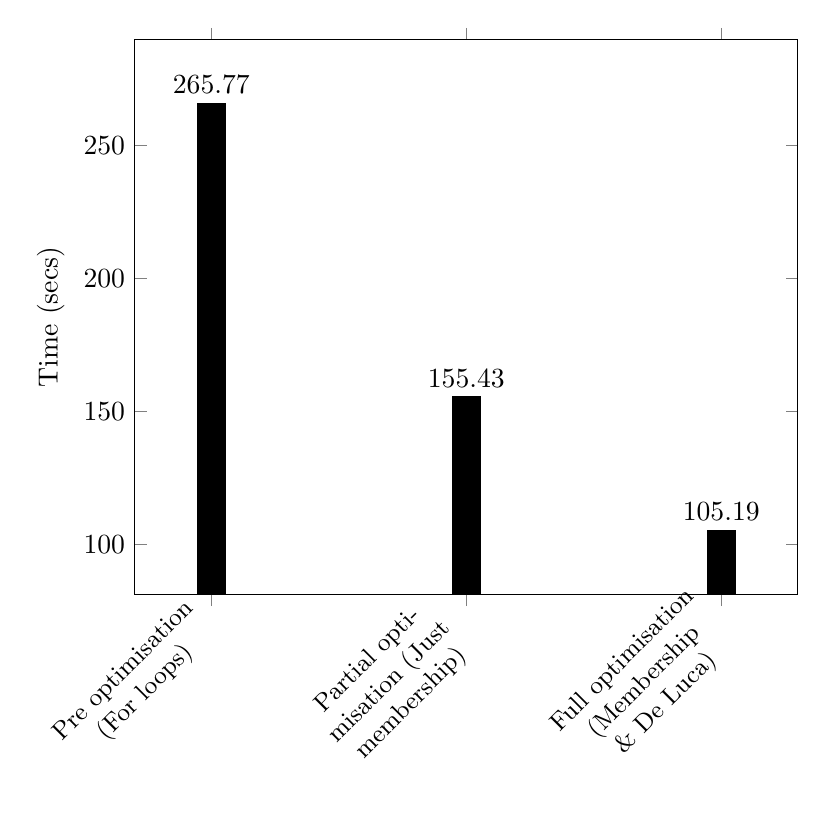
\begin{tikzpicture}
      \begin{axis}[
        width= 10cm,
        symbolic x coords={Pre optimisation (For loops),Partial optimisation (Just membership),Full optimisation (Membership \& De Luca)},
        x tick label style={font=\small,text width=2.5cm,align=center},
        ybar,
        enlargelimits=0.15,
        legend style={at={(0.5,-0.2)},
          anchor=north,legend columns=-1},
        ylabel={Time (secs)},
        xtick={Pre optimisation (For loops),Partial optimisation (Just membership),Full optimisation (Membership \& De Luca)},
        nodes near coords,
    	  nodes near coords align={vertical},
        x tick label style={rotate=45,anchor=east},
        ]
        \addplot[ybar,fill] coordinates {
    (Pre optimisation (For loops),265.771186)
    (Partial optimisation (Just membership),155.432352)
    (Full optimisation (Membership \& De Luca),105.188263) };
      \end{axis}
    \end{tikzpicture}
    \caption{A comparison of the total time to run 5 iterations prior to vectorisation, during (part vectorisation) and post-vectorisation.}
    \label{fig:total-time}
  \end{center}
\end{figure}

Figure \ref{fig:total-time} outlines the total time taken to run 5 iterations of Non-Probabilistic Entropy before vectorisation, once vectorisation was complete on the \texttt{membership.m} function, and finally after full vectorisation.
